\documentclass[12pt]{article}
\usepackage{amssymb}
%\usepackage[UTF8]{ctex}
\usepackage{amsmath}
\usepackage{amsthm}
\usepackage{geometry}
\usepackage{booktabs}
\usepackage{bm}
\usepackage{cite}
%\usepackage{CJK}
\usepackage[many]{tcolorbox}
%\tcbuselibrary{listingsutf8}
%\tcbuselibrary{skins, breakable, theorems, most}
%\geometry{a4paper,bottom = 3cm,left = 3cm, right = 3cm}

%for reference
\usepackage{hyperref}
\usepackage[capitalise]{cleveref}
\crefname{enumi}{}{}

\newtheorem{theorem}{Theorem}
\newtheorem{lemma}[theorem]{Lemma}
\newtheorem{proposition}[theorem]{Proposition}
\newtheorem{question}[theorem]{Question}
\newtheorem{definition}[theorem]{Definition}
\newtheorem*{remark}{Remark}
%\newenvironment{proof}{\noindent \textbf{Proof:}}{$\Box$}

%to use newcommand for convenience
\newcommand\field{\mathbb{F}}
\newcommand\R{\mathbb{R}}
\newcommand\Q{\mathbb{Q}}
\newcommand\Z{\mathbb{Z}}
\newcommand\N{\mathbb{N}}
\newcommand\cc{\mathcal{C}}
\newcommand\bb{\mathcal{B}}
\newcommand\pp{\mathcal{P}}
\newcommand\nn{\mathcal{N}}
\newcommand\ff{\mathcal{F}}
\newcommand\one{\bm{1}}
\newcommand\eps{\varepsilon}
\newcommand\pr[1]{\mathcal{P} \left( #1\right)}
\DeclareMathOperator{\leb}{Leb}   
\DeclareMathOperator{\diff}{d}   

\title{An Application of Lovász Local Lemma: Hypergraph 2-Coloring}
\author{Xinyu Mao}
\date{\today}
\begin{document}
\maketitle
During the lecture, we have established \textbf{Lovász Local Lemma}:
\begin{lemma}[Erdös,Lovász, 1975] \label{LLL}
    Let $E_1,E_2,\dots,E_n$ be a sequence of events 
    on some probability space $(\Omega, \Sigma, \pp)$
    with $\pp(E_i) \leq p$ for all $i \in [n]$ and 
    all degrees in dependency graph $G = (V,E)$ are at most $d$.
    If $4pd \leq 1$, then 
    $$
        \pr{\bigcap_{i = 1}^n E_i^c} > 0.
    $$
\end{lemma}
The above lemma provides a deeper insight into many combinatorics problems, 
in particular to give existence proofs.  
We learned about $k$-sat problem in the lecture, 
and another application is \textbf{Hypergraph 2-Coloring}.

\begin{definition}
    A hypergraph $H$ is a pair $H = (X,E)$ 
    where $X$ is a set of elements called vertices, and 
    $E$ is a set of non-empty subsets of $X$ called hyperedges or edges.
\end{definition}
Intuitively, a hypergraph is a generalization of a graph where an edge 
consists of any number of vertices.
And the Hypergraph 2-Coloring problem is
\begin{question}
    Given a hypergraph $H$, can we assign two colors to vertices
    so that no edge is monochromatic?
\end{question}
We say $H$ is \textit{2-colorable} if the answer is yes. For example, the hypergraph in \cref{ex}(a) is 2-colorable,
while \cref{ex}(b) is not.
\begin{figure}[h]
    \centering
    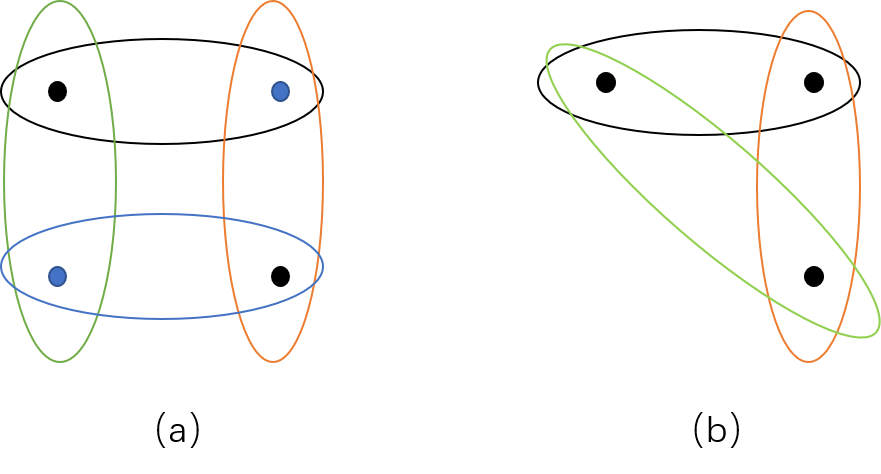
\includegraphics[width = 0.7\textwidth]{ex.png}
    \caption{Example of 2-coloring of hypergraph.}
    \label{ex}
\end{figure} 

With the help of \cref{LLL}, we can prove that 
\begin{theorem}
    Let $H = (X,E)$ be a hypergraph in which every 
    edge has at least $k$ vertices and 
    intersects at most $d$ other edges.
    If $4d \leq 2^{k - 1}$, then $H$ is 2-colorable.
\end{theorem}
\begin{proof}
Let $E = \{e_1,e_2,\dots,e_n\}$. 
We color the vertices randomly
and define $E_i$ as the event that edge $e_i$ is monochromatic.
Clearly, $\pp(E_i) \leq \frac{1}{2^{k-1}}$ for all $i \in [n]$
and the degree in dependency graph is at most $d$.
Take $p = \frac{1}{2^{k-1}}$ and we have 
$4pd \leq 1$. Hence, by \cref{LLL} we get
$$
    \pr{\bigcap_{i=1}^n E_i^c} > 0,
$$
which means $H$ is 2-colorable.
\end{proof}

Another application of \cref{LLL} is 
\textbf{package routing}.
To find the optimal solution is NP-hard, but with the help of
\textit{the algorithmic
version of the Lovasz Local Lemma}(I did not look into this in detail...),
we can design and validate some good schedules\cite{leighton1994packet}.

\bibliographystyle{unsrt}
\bibliography{ref.bib}
\end{document}